\chapter{Аналитическая часть}

В данном разделе будут изучены основы теории графов, а также будет выбран способ представления графа. Кроме того, будет описан алгоритм Флойда поиска кратчайших расстояний между всеми парами вершин графа.

\section{Основы теории графов}

Многие объекты, возникающие в жизни человека, могут быть смоделированы (представлены в памяти компьютера) при помощи графов. Например, транспортные схемы (схема метрополитена и т. д.) изображают в виде станций, соединенных линиями. В терминах графов станции называются вершинами графа, а линии – ребра.

Графом \cite{graph} называется конечное множество вершин и множество ребер. Каждому ребру сопоставлены две вершины – концы ребра. Число вершин графа называют порядком. Путем на графе называется последовательность ребер, в которой конец одного ребра является началом следующего ребра. Начало первого ребра называется началом пути, конец последнего ребра - концом пути.

Бывают различные варианты определения графа. В данном определении концы у каждого ребра – равноправны. В этом случае нет разницы где начало, а где – конец у ребра. Но, например, в транспортных сетях бывают случаи одностороннего движения по ребру, тогда говорят об ориентированном графе – графе, у ребер которого одна вершина считается начальной, а другая – конечной.

Очень часто рассматриваются графы, в которых каждому ребру приписана некоторая числовая характеристика – вес. Вес может означать длину дороги или стоимость проезда по данному маршруту. Соответствующие графы называются взвешенными.

\subsection{Способы представления графов}

Представление графов в памяти – это способ хранения информации о ребрах графа, позволяющий решать следующие задачи:

\begin{itemize}
	\item для двух данных вершин проверить, соединены ли вершины ребром;
	\item перебрать все ребра, исходящие из данной вершины.
\end{itemize}

Существует два способа представления графа. Рассмотрим их далее для следующего графа:

\begin{figure}[H]
	\begin{center}
		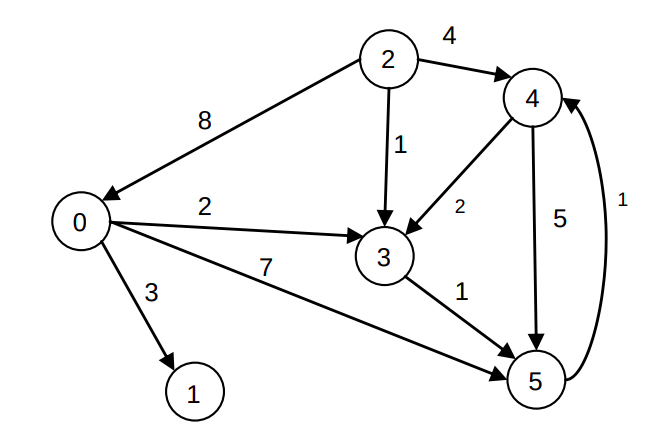
\includegraphics[scale=0.5]{img/graph.png}
	\end{center}
	\captionsetup{justification=centering}
	\caption{Ориентированный взвешенный граф}
	\label{img:graph}
\end{figure}

\subsubsection{Списки смежности}

При представлении графа списками смежности для каждой вершины i хранится список W[i] смежных с ней вершин. Для рассмотренного примера списки будут такими:

\clearpage

$W[1] = [2, 4, 6]$

$W[2] = [ ]$

$W[3] = [1, 4, 5]$

$W[4] = [6]$

$W[5] = [4, 6]$

$W[6] = [5]$

Таким образом, весь граф можно представить одним списком, состоящим из вложенных списков смежности вершин.

При представлении взвешенного графа списками смежности можно поступить двумя способами. Можно в списках смежности хранить пару (кортеж) из двух элементов – номер конечной вершины и вес ребра. Но в этом случае неудобно проверять наличие ребра между двумя вершинами.

Другой способ – хранить списки смежности как ранее, а веса ребер хранить в отдельном ассоциативном массиве, в котором ключом будет пара из двух номеров вершин (номер начальной и конечной вершины), а значением будет вес ребра между этими вершинами.

\subsubsection{Матрица смежности}

При представлении взвешенного графа матрицей смежности информация о ребрах графа хранится в квадратной матрице (двумерном списке), где элемент A[i][j] равен весу ребра, если ребра i и j соединены ребром.  Иначе равен определенному символу (для рассматриваемого графа -1):

\begin{equation}
	A = \begin{pmatrix}
		0 & 3 & -1 & 2 & -1 & 7\\
		-1 & 0 & -1 & -1 & -1 & -1\\
		8 & -1 & 0 & 1 & 4 & -1\\
		-1 & -1 & -1 & 0 & -1 & 1\\
		-1 & -1 & -1 & 2 & 0 & 5\\
		-1 & -1 & -1 & -1 & 1 & 0\\
	\end{pmatrix}
\end{equation}

Если граф не является взвешенным, то элемент матрицы смежности равен 1, если ребра соединены.

Матрица смежности требует $O(n^2)$ памяти и может оказаться неэффективным способом хранения дерева или разреженных графов. Но использование матрицы смежности позволяет применять при реализации вычислительных процедур анализа графов матричные
алгоритмы обработки данных, которые можно распараллелить. Поэтому при реализации данной лабораторной работы граф будет представляться при помощи матрицы смежности.

\section{Алгоритм Флойда}

Алгоритм Флойда \cite{alg} позволяет найти кратчайшее расстояние между любыми двумя вершинами в графе.

\subsection{Последовательный алгоритм}

Будем считать, что в графе $n$ вершин, пронумерованных числами от $0$ до $n - 1$. Граф задан матрицей смежности, вес ребра $i - j$ равен $w_{ij}$. При отсутствии ребра $i - j$ значение $w_{ij} = -1$, также будем считать, что $w_{ii} = 0$.

Пусть значение $a^k_{ij}$ равно длине кратчайшего пути из вершины $i$ в вершину $j$, при этом путь может заходить в промежуточные вершины только с номерами меньшими $k$ (не считая начала и конца пути). То есть $a^0_{ij}$ - это длина кратчайшего пути из $i$ в $j$, который вообще не содержит промежуточных вершин, то есть состоит только из одного ребра $i - j$, поэтому $a^0_{ij} = w_{ij}$. Значение $a^1_{ij} = w_{ij}$ равно длине кратчайшего пути, который может проходить через промежуточную вершину с номером 0, путь с весом $a^2_{ij}$ может проходить через промежуточные вершины с номерами 0 и 1 и т. д. Путь с весом $a^n_{ij}$ может проходить через любые промежуточные вершины, поэтому значение $a^n_{ij}$ равно длине кратчайшего пути из $i$ в $j$.

Алгоритм Флойда последовательно вычисляет $a^0_{ij}$, $a^1_{ij}$, $a^2_{ij}$, …, $a^n_{ij}$, увеличивая значение параметра $k$. Начальное значение - $a^0_{ij} = w_{ij}$.

Теперь предполагая, что известны значения $a^{k - 1}_{ij}$ вычислим $a^k_{ij}$. Кратчайший путь из вершины $i$ в вершину $j$, проходящий через вершины с номерами, меньшими, чем $k$ может либо содержать, либо не содержать вершину с номером $k - 1$. Если он не содержит вершину с номером $k - 1$, то вес этого пути совпадает с $a^{k - 1}_{ij}$. Если же он содержит вершину $k - 1$, то этот путь разбивается на две части: $i - (k - 1)$ и $(k - 1) - j$. Каждая из этих частей содержит промежуточные вершины только с номерами, меньшими $k - 1$, поэтому вес такого пути равен $a^{k - 1}_{i,k-1} + a^{k - 1}_{k-1,i}$. Из двух рассматриваемых вариантов необходимо выбрать вариант наименьшей стоимости, поэтому:

\begin{equation}
	a^k_{ij} = min(a^{k - 1}_{ij}, a^{k - 1}_{i,k-1} + a^{k - 1}_{k-1,i})
\end{equation}

\subsection{Параллельный алгоритм}

Более эффективный способ алгоритма может состоять в одновременном выполнении нескольких операций обновления значений матрицы смежности A. Параллельный алгоритм Флойда заключается в том, что на k-й итерации мы отсылаем k-ю строку всем процессам, а затем каждый процесс выполняет последовательный алгоритм Флойда для полосы матрицы смежности, одновременно обновляя значение матрицы.

\section{Вывод}

Были изучены основы теории графов и способы представления графа. Граф будет представляться при помощи матрицы смежности. Также были рассмотрены последовательный и параллельный варианты алгоритма Флойда поиска кратчайших путей между всеми парами вершин графа.

Программе, реализующей данный алгоритм, на вход будет подаваться матрица смежности, которая задает граф. Выходными данными такой программы должна быть матрица смежности кратчайших путей между всеми парами вершин графа. Программа должна работать в рамках следующих ограничений:

\begin{itemize}
	\item веса ребер графа - целые неотрицательные числа;
	\item осутствие пути между вершинами обозначается -1;
	\item порядок графа должен быть больше, либо равен 2;
	\item должно быть выдано сообщение об ошибке при вводе пустой матрицы смежности или при вводе недопустимого веса ребра графа.
\end{itemize}

Пользователь должен иметь возможность выбора построения алгоритма с распараллеливанием и без него. В случае параллельного алгоритма пользователь должен иметь возможность ввода числа потоков. Также должны быть реализованы сравнение алгоритмов по времени работы в зависимости от числа потоков и в зависимости от порядка графа с выводом результатов на экран и получение графического представления результатов сравнения. Результат данных действий пользователь должен получать при помощи меню.